\documentclass[../main/main.tex]{subfiles}


\begin{document}

\section{March 11th, 2021}
\subsection{Properties of Conjugate Gradient}
Going back to the projection framework, we know that CG is derived from 2-dim projection method by choosing $K = \sspan \{r_{k}, d_{k-1}\}$.
\begin{theorem}
CG is a $K$-dim projection method at step $K$.
\end{theorem}
  Since
  \begin{align*}
x_{k+1} &= \argmin _{x\in x_{k}+\sspan \{r_{k},d_{k-1}\}} \|x_{*}-x\|_{A}
    .\end{align*}
  The residue vector must be orthogonal to the subspace, meaning:
  \begin{align*}
    \iprod{x_{*}-x_{k+1}}{v} &= 0 \quad  \forall  v \in \sspan \{r_{k},d_{k-1}\}\\
   \iff   \iprod{r_{k+1}}{v} &= 0
    .\end{align*}
  Therefore:
  \begin{align*}
& \iprod{r_{k+1}}{r_{k}}= 0, \quad \iprod{r_{k+1}}{d_{k-1}}=0, \quad \iprod{r_{k+1}}{d_{k}} = 0
    .\end{align*}
  Thus, with $\alpha _{k}\neq 0$ (i.e. $r_{k}\neq 0$), $\beta _{k}$ is optimal in the sense that:
  \begin{align*}
    &\beta _{k} = \argmin_{\beta \in \RR }  \|x_{k}+\alpha _{k}(r_{k}+\beta d_{k-1})-x_{*}\|_{A}\\
    \iff & d_{k} = \argmin_{d\in r_{k}+\sspan \{d_{k-1}\}} \|x_{k}+\alpha _{k}d - x_{*}\|_{A}\\
    \iff & d_{k} = \argmin_{d\in r_{k}+\sspan \{d_{k-1}\}} \left\|d - \frac{1}{\alpha _{k}}(x_{*}-x_{k})\right\|_{A}
    .\end{align*}
  Thus $d_{k}$ is the projection of $\frac{1}{\alpha _{k}}(x_{*}-x_{k})$ onto the 1-dim subspace $r_{k}+\sspan \{d_{k-1}\}$. As such, we have:
  \begin{align*}
    &\iprod{d_{k-1}}{d_{k}-\frac{1}{\alpha _{k}}(x_{*}-x_{k})}_{A}=0\\
    & \iprod{d_{k-1}}{d_{k}}_{A} = \frac{1}{\alpha _{k}}\iprod{d_{k-1}}{x_{*}-x_{k}}_{A} = \frac{1}{\alpha _{k}}\iprod{d_{k-1}}{r_{k}} = 0
      .\end{align*} since $\iprod{r_{k+1}}{d_{k}}=0$. As such: \[
      \iprod{d_{k-1}}{d_{k}}_{A}=0, \quad  if r_{k}\neq 0
    \] which means that each $d_{k}$ is orthogonal from $d_{k-1}$.
    \begin{remark}
If $r_{k}=0$, then the algorithm stops, since we have achieved $x_{*}$.
    \end{remark}
    In general $a\perp b, b\perp c\centernot\implies a\perp c$, since orthogonality is not transitive. However, the orthogonality of vector produced by CG is transitive.
    \begin{figure}[htpb]
      \centering
      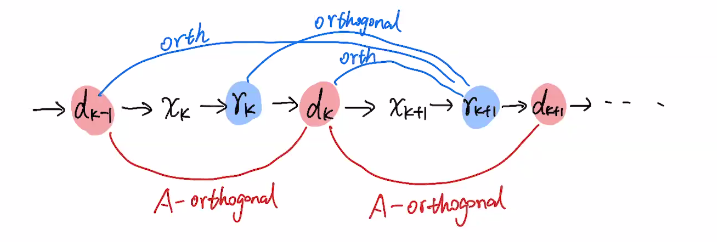
\includegraphics[width=0.8\textwidth]{../images/3-11-orth.png}
      \caption{Diagram showing Orthogonality between $d_{k}$ and $r_{k}$ }
    \end{figure}
    \begin{theorem}
      Assume $A$ is SPD. Assume $r_{0},r_1,r_2, \ldots ,r_{i-1}\neq 0$. Then:
      \begin{enumerate}
\item $\iprod{r_{j}}{r_{j}} = 0$ for all $j\leq  i-1$ (meaning $\{r_{0},r_{1}, \ldots , r_{i}\}$ are orthogonal)
        \item
              \begin{enumerate}
\item $\iprod{r_{i}}{d_{j}}=0$ for all $j\leq  i-1$
\item $\iprod{r_{i}}{d_{j}}_{A}=0$ for all $j\leq  i-2$
\item $\iprod{d_{i}}{r_{j}}_{A}=0$ for all $j\leq  i-1$
              \end{enumerate}
              \item $\iprod{d_{i}}{d_{j}}_{A}=0$ for all $j\leq i-1$ ($\{d_{0},d_{1}, \ldots , d_{i}\}$ are $A$-orthogonal)
      \end{enumerate}
    \end{theorem}

    \begin{proof}
By Induction. Check notes.
    \end{proof}
    In matrix form, this is equivalent to:
    \begin{enumerate}
\item $\iff $ Let $R_{i}= \begin{bmatrix}
r_{0}&r_{1}& \ldots &r_{i}
\end{bmatrix}\in \RR ^{n \times (i+1)}$. Then:$R_{i}^{T}R_{i}$ is diagonal.
\item $\iff $ Let $D_{i}= \begin{bmatrix}
d_{0}&d_{1}& \ldots &d_{i}
\end{bmatrix}\in \RR ^{n \times (i+1)}$. Then:
\begin{enumerate}
  \item $R_{i}^{T}D_{i}$ is  $\begin{bmatrix}
\times   &\ldots &\times \\
 & \ddots&\vdots\\
 0& &\times \\
  \end{bmatrix}$, i.e. upper triangular.

  \item $R_{i}^{T}AD_{i}$ is  $\begin{bmatrix}
    \times  &&&& \\
    \times  &\times &&& \\
      &\times  &\ddots&& \\
      &&\ddots &\ddots& \\
      &&&\times &\times \\
  \end{bmatrix}$, i.e. upper triangular.
\end{enumerate}
\item $\iff D_{i}^{T}A D_{i}$ is diagonal.
    \end{enumerate}
\begin{theorem}\label{3-11-k}
  $\{x_{k}\}$ generated by CG satisfies: \[
\iprod{x_{*}-x_{k}}{v}_{A}=0 \quad \forall v\in K_{k}
\] where $K_{k}$ is the Krylov subspace. As a result: \[
x_{k} = \argmin_{x\in x_{0}+K_{k}}  \|x_{*}-x\|_{A}\]
\end{theorem}
\begin{definition}[\vocab{Krylov Subspace}]\index{Krylov subspace}
  \[
    K_{k}\coloneqq \sspan \{r_{0}, Ar_{0}, A^2r_{0}, \ldots ,A^{k-1}r_{0}\}
  \]
\end{definition}
\begin{figure}[htpb]
  \centering
  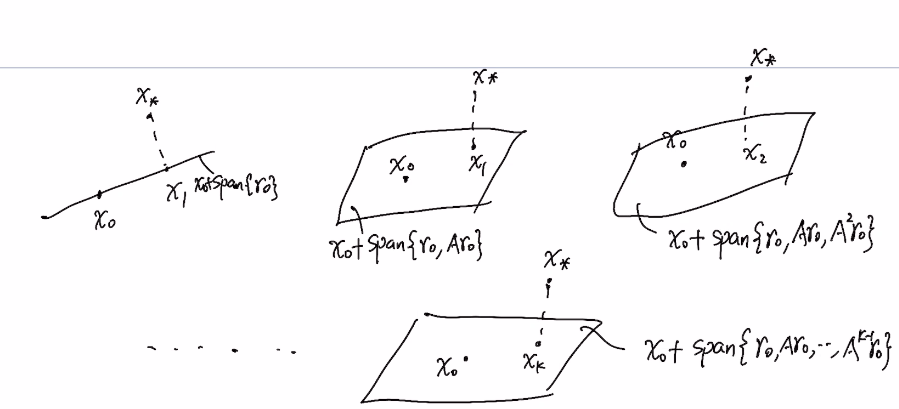
\includegraphics[width=0.8\textwidth]{../images/3-11-k.png}
  \caption{Pictoral Representation of Theorem \ref{3-11-k}}
\end{figure}
\begin{proof}

\end{proof}
\begin{corollary}
If we run CG for $N$ steps, it is equivalent to projecting to $\RR ^{n}$, which is $x_{*}$, thus meaning that CG is optimal.
\end{corollary}
\end{document}
